% This file was created with tikzplotlib v0.10.1.
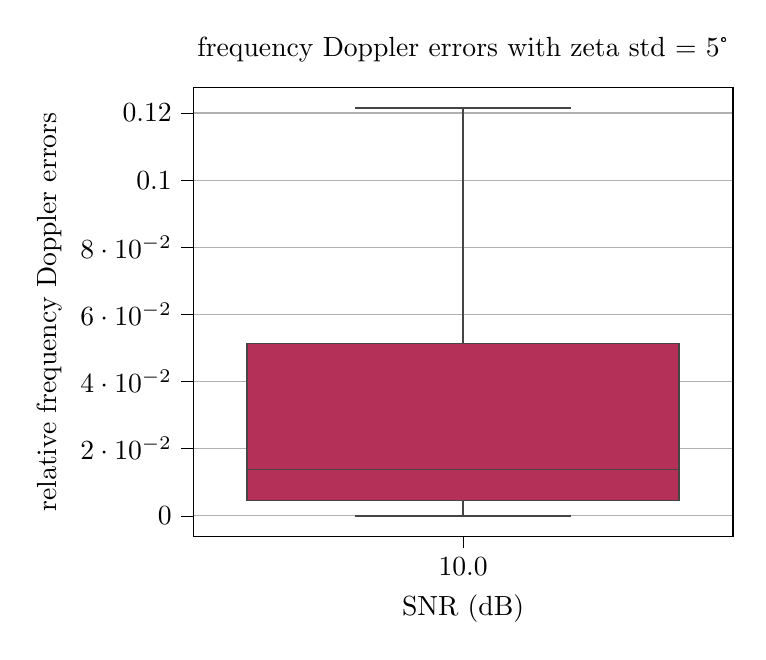
\begin{tikzpicture}

\definecolor{brown1814888}{RGB}{181,48,88}
\definecolor{darkgray176}{RGB}{176,176,176}
\definecolor{darkslategray69}{RGB}{69,69,69}

\begin{axis}[
tick align=outside,
tick pos=left,
title={frequency Doppler errors with zeta std = 5°},
x grid style={darkgray176},
xlabel={SNR (dB)},
xmin=-0.5, xmax=0.5,
xtick style={color=black},
xtick={0},
xticklabels={10.0},
y grid style={darkgray176},
ylabel={relative frequency Doppler errors},
ymajorgrids,
ymin=-0.00606936005324245, ymax=0.127484379982049,
ytick style={color=black}
]
\path [draw=darkslategray69, fill=brown1814888, semithick]
(axis cs:-0.4,0.0045579040415196)
--(axis cs:0.4,0.0045579040415196)
--(axis cs:0.4,0.0513097834455038)
--(axis cs:-0.4,0.0513097834455038)
--(axis cs:-0.4,0.0045579040415196)
--cycle;
\addplot [semithick, darkslategray69]
table {%
0 0.0045579040415196
0 1.26449381624788e-06
};
\addplot [semithick, darkslategray69]
table {%
0 0.0513097834455038
0 0.12141375543499
};
\addplot [semithick, darkslategray69]
table {%
-0.2 1.26449381624788e-06
0.2 1.26449381624788e-06
};
\addplot [semithick, darkslategray69]
table {%
-0.2 0.12141375543499
0.2 0.12141375543499
};
\addplot [semithick, darkslategray69]
table {%
-0.4 0.0137588699030109
0.4 0.0137588699030109
};
\end{axis}

\end{tikzpicture}
